\section{Experimental results}
\label{sec:results}

\noindent\textbf{Setup.} Every table and figure applies the procedure of Sec.~\ref{sec:method} to released
checkpoints or training-free baselines; the reproduction is in Sec.~\ref{sec:discussion}. We use the Sony sRGB extreme-dark benchmark derived from SID~\cite{sid2018} in the
processed sRGB form prepared for SNR-Net~\cite{snrnet2022} and released with
Retinexformer~\cite{retinexformer}: \nNSCENE{} test scenes and \nNIMG{} short-exposure frames
at $512\times960$, each scored against the single long-exposure frame of its scene. As a
standard low-light benchmark we use LOL~\cite{lol2018} ($15$ test frames) with its v2
sets~\cite{lolv2_2021}. The model under analysis is the released Retinexformer checkpoint; inference is
deterministic, so every spread is over frames or scenes. We reproduce its reported score
to within \(0.002\) dB with our own metric implementation (Sec.~\ref{sec:discussion}).



\IfFileExists{tab_cmp_rows.tex}{%
\begin{table}[t]
\centering\caption{Existing methods under one protocol (rounding, no rectification) and the decomposition
of each residual (rightmost four columns): PSNR in dB (mean$\pm$sd over frames; $15$ on LOL, $598$ on Sony), SSIM, squared-error shares in percent (pooled over frames) removed by the global gain,
the per-channel gain and the remainder, and $\Delta_{16}$ in dB (frame mean), the control-corrected
$16$-pixel block-gain ceiling over the whole-frame gain. Diffusion models: one sample, fixed seed (LightenDiffusion's seed spread \nLDspread{}\,dB). URetinex-Net: fixed ratio (its published score uses a reference-derived ratio). GSAD: published \nGSADpub{} is rectified (\nGSADrect{} here). Zero-DCE++:
run on the 12-multiple crop its code requires, curve map edge-extended. AR: in-house Retinex model, self-supervised on COCO. Gamma 0.5 and the perceptual-loss CIDNet variant appear only in the released
comparison table. Rows: by benchmark; reference-free methods first, then reference-trained ones by year; Sony rows: methods with a Sony checkpoint or none needed. LOL per-frame sd: shares up to \nLOLshareSDmax{} points, $\Delta_{16}$ up to \nLOLdSDmax{}\,dB.}
\label{tab:decomp}
\setlength{\tabcolsep}{3.2pt}
\begin{tabular}{lcccccc}
\toprule
method & PSNR & SSIM & gl. & ch. & res. & $\Delta_{16}$ \\
\midrule
\inputrows{tab_cmp_rows.tex}
\bottomrule
\end{tabular}
\end{table}}{}
\IfFileExists{fig_cmp_sony.pdf}{%
\begin{figure*}[t]
\centering
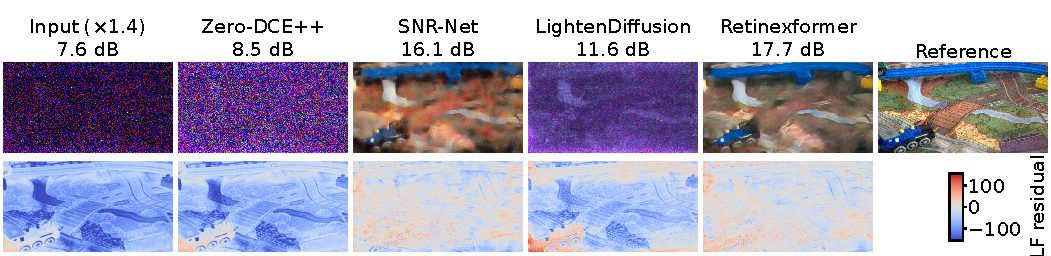
\includegraphics[width=\textwidth]{fig_cmp_sony.pdf}
\caption{Existing methods on the $0.033$\,s Sony frame on which Retinexformer scores lowest: input after its oracle global gain (label: score before it), four outputs, and the reference (top); the decomposition applied to input and methods: the low-frequency part (below
$0.10$) of each residual after its own oracle global gain (bottom, common 8-bit range). Every method leaves a spatially varying brightness field of method-specific size.}
\label{fig:cmp}
\end{figure*}}{}

\noindent\textbf{Existing methods under one protocol, and the proposed decomposition
applied to each.} Table~\ref{tab:decomp} scores, with rounding and no rectification, the outputs of \nCMPnLOL{} methods on LOL and \nCMPnSony{} on Sony: CLAHE~\cite{clahe1994},
the zero-reference Zero-DCE++~\cite{zerodcepp2022}, SCI~\cite{sci2022} (released weights trained on LOL and LSRW), an in-house self-supervised Retinex model (AR), the unsupervised diffusion model
LightenDiffusion~\cite{lightendiff2024} (unpaired training on LSRW, not evaluated on Sony
by its authors), and networks trained on each benchmark with its reference
(URetinex-Net~\cite{uretinex2022}, SNR-Net~\cite{snrnet2022}, LLFormer~\cite{llformer2023},
the diffusion model GSAD~\cite{gsad2023}, Retinexformer, CIDNet~\cite{cidnet}); the rightmost four columns are Sec.~\ref{sec:method} applied to each method's own residual; Fig.~\ref{fig:cmp} shows
one frame. On LOL \nCMPclearLOL{} methods clear $20$\,dB unrectified: the reference-trained
networks other than URetinex-Net with its fixed ratio, and LightenDiffusion at
\nLDlol{}, a count that its sampling spread can lower to five; the rest stay below
\nCMPrestLOL{}\,dB. On Sony only the two trained on it, SNR-Net and Retinexformer, clear $20$\,dB, and
LightenDiffusion leaves \nLDsonyChan{} percent of its error in the per-channel term, a colour cast. Across the enhancement methods in Table~\ref{tab:decomp} (bounds rounded outward) the
global term ranges from
\nCMPglobLOLlo{} to \nCMPglobLOLhi{} percent of the error on LOL and from
\nCMPglobSonylo{} to \nCMPglobSonyhi{} on Sony, so which term dominates varies with method and benchmark, while the block
ceiling stays between \nCMPdLOLlo{} and \nCMPdLOLhi{}\,dB on LOL and
\nCMPdSonylo{} and \nCMPdSonyhi{}\,dB on Sony: the spatially varying low-frequency term is
common to all.

\noindent\textbf{Global tone and colour: a priced ceiling, not an exhausted one.} On Sony an oracle global gain and per-channel gain account for \nSHAREglob{} and
\nSHAREchan{} percent of Retinexformer's squared error, taking the score from \nPSNRmodel{} to \nPSNRchan{} dB;
the remaining \nSHAREresid{} percent survives any global or per-channel gain, growing from \nSHAREresidLong{} percent at $0.1$\,s to \nSHAREresidShort{} at $0.033$\,s.
\IfFileExists{tab_cmp_rows.tex}{}{%
\begin{table}[t]
\centering\caption{Decomposition across benchmarks and architectures. Shares are percentages of
squared error; $\Delta_{16}$ is the control-corrected gain of a per-block gain oracle at
$16$ pixels; LF is the share of error energy below $0.10$. LOL is $15$ frames.}
\label{tab:decomp}
\setlength{\tabcolsep}{3.0pt}
\begin{tabular}{llcccccc}
\toprule
data & method & PSNR & glob. & chan. & resid. & $\Delta_{16}$ \\
\midrule
\inputrows{tab_cross_rows.tex}
\bottomrule
\end{tabular}
\end{table}}


\noindent\textbf{The structural term is decorrelation, not attenuation.} Output power falls with radial frequency (ratio \nPOWlow{} in the lowest band,
\nPOWhigh{} at the corner), and the output is closer to a blurred reference than to the
reference: with $\sigma=\nBLURsigma{}$ the output scores \nBLURpsnr{} dB against
the blurred reference, \nBLURdelta{} dB above its gain-corrected score against the reference (\nBLURbase{}),
which is the signature of a conditional-mean solution~\cite{blau2018}. Restoring the lost amplitude buys almost nothing: rescaling each band of the output to the
reference power with its own phase moves the score by \nAMPdelta{} dB, the least-squares
per-band gain by \nBANDLSdelta{} dB, because $\rho_j$ falls from near unity in the lowest
band to \nRHOshortcorner{} at the corner for the shortest exposure.

\begin{table}[t]
\centering\caption{Band-wise correlation with the reference: model output against scalar brightness-matched
input (Sec.~\ref{sec:method} primary path, all frames); conservative in the model's favour, the text gives the noise-corrected reading;
\dag{} marks unstable input cells ($N_j/P_j>0.9$).}
\label{tab:rho}
\setlength{\tabcolsep}{3.5pt}
\begin{tabular}{lcccccc}
\toprule & \multicolumn{2}{c}{0.033\,s ($n=\nNshort{}$)} & \multicolumn{2}{c}{0.04\,s ($n=\nNmid{}$)} & \multicolumn{2}{c}{0.1\,s ($n=\nNlong{}$)}\\
band & model & input & model & input & model & input \\
\midrule
\inputrows{tab_rho_rows.tex}
\bottomrule
\end{tabular}
\end{table}



\noindent\textbf{Two readings, stated together.} Against the brightness-matched input the
model's correlation is at or above it in every band and at every exposure
(Table~\ref{tab:rho}), so no band is recoverable under that criterion; at $0.033$\,s \nRAWunshort{} percent of the
error sits in bands where the input's own agreement is below the floor. Under the noise-corrected ceiling of Sec.~\ref{sec:method} the
recoverable share is \nSCALrecshort{}, \nSCALrecmid{} and \nSCALreclong{} percent at
$0.033$, $0.04$ and $0.1$\,s. Corrected cells with $N_j/P_j>0.9$, the bands above normalised frequency \nNPshortFrom{}
at $0.033$\,s and above \nNPmidFrom{} at $0.04$\,s, are read as unstable; the $0.04$\,s share of \nSCALrecmid{} percent comes entirely from one such cell ($N_j/P_j=\nNPmidCorner{}$), the $0.1$\,s share from a
stable one. The verdict is margin-sensitive: at margin zero the three shares become \nMZrecshort{},
\nMZrecmid{} and \nMZreclong{} percent, \nMZunshort{} and \nMZunmid{} points of which come
from those unstable cells, and the two bands that clear the $0.05$ margin exceed it by
\nEXmid{} and \nEXlong{}. The
additive-noise assumption behind the correction was tested on the same captures: on this
scalar path it passes the aggregate checks and fails the lowest-band check at $0.04$ and
$0.1$\,s (not run at $0.033$\,s, two frames per scene), where the
noise estimate is small and the output correlation exceeds $0.99$, so no verdict can
change. It fails at low frequency on the alternative pointwise path, which fits a per-frame tone
curve to the reference and hands the input information it does not have; there the shares
rise to \nPWrecshort{}, \nPWrecmid{} and \nPWreclong{} percent, an
optimistic bound.

\noindent\textbf{This single-frame checkpoint cannot consume a burst.} The natural way to
spend the multi-frame margin is to average $k$ input frames. On
the \nMFn{} scene--exposure groups with at least eight frames ($36$ at $0.1$\,s, $14$ at $0.04$\,s), so that every $k$ is scored on identical
groups, this raises the low-frequency error energy after the oracle global gain
monotonically, to \nMFlfb{}, \nMFlfd{} and \nMFlfh{} times the single-frame value at
$k=2$, $4$ and $8$, where pure variance would have given $1/k$, while the high-frequency
energy falls only to \nMFhfh{}. On the \nMFlongN{} scenes at $0.1$\,s the raw score of the
eight-frame mean falls by \nMFinDrop{} dB, yet on the same $36$ groups the input's own band correlation (all $361$ frames of those groups, then their $36$ eight-frame means) rises in every band, at the corner from \nMFinFixA{} to
\nMFinFixB{}, and the model's on the averaged input (eight frames per group) in nine of
eleven (the lowest two fall), at the corner from \nMFrhoA{} to \nMFrhoB{}, so
the structure improves and the brightness field collapses. Averaging the model's outputs instead of its inputs gains
\nMFoutGain{} dB at $k=8$; the noise-realisation share (half the mean squared difference between outputs of two
frames of one scene and exposure over the model's squared error) is \nNOISEshare{} percent, \nNOISEdb{} dB, on the full test set under an independence
assumption. A noise-variance frequency-domain burst merge~\cite{hdrplus2016}, on all \nHPn{} groups at $k=8$ with the
noise level estimated from the frames, scores \nHPFe{} dB
against \nHPB{} (plain mean) and \nHPA{} (one frame): it recovers \nHPdFB{} dB of what
the mean loses, almost all below $0.05$ normalised frequency, and stays \nHPdFA{} dB
below a single frame. The dominant term is a frame-common bias, not the model reading noise level as a
brightness cue: re-injecting noise into the eight-frame mean moves the
low-frequency error to \nNCmatch{} and adding noise to a single frame to \nNCextra{}; the checkpoint's low-frequency
estimate is tuned to its training statistics and departs from the reference either way.


\noindent\textbf{What carries over to the second benchmark.} Three findings carry over from Sony to LOL: the output again closer to a blurred
reference; the low-frequency part again dominant, \nLOLlfLo{} to \nLOLlfHi{} percent of
the error energy; and the block oracle again above a decibel, \nLOLladCID{} and
\nLOLladRET{}\,dB at $16$ pixels ($\Delta_{16}$ in Table~\ref{tab:decomp}), of which a control fitted to another frame's residual takes \nLPcidPerm{}
and \nLPretPerm{}\,dB, \nLPcidPct{} and \nLPretPct{} percent of them against
\nPERMpctC{} percent on Sony, so about a quarter of the LOL block ceiling is frame-specific, on Sony
almost none. Hygiene check: all eleven LOL bands are exhausted against the raw input for both CIDNet
variants and Retinexformer.

\noindent\textbf{The dominant term is a spatially varying low-frequency field.} The residual after the
global gain is concentrated at low frequency: the low-pass part carries \nLFshare{}
percent of the error energy, of which a single per-frame constant explains only
\nLFconst{} percent. Fig.~\ref{fig:workflow} prices it: an oracle allowed one scalar per $16$-pixel block gains \nLADgain{} dB over the whole-frame fit, an offset per block \nLADoff{} dB, and an affine map per block \nLADaff{} dB, after subtracting the structureless-target control, which is negligible. A second, more demanding control, fitting the same block gains to another frame's
residual of matched variance, recovers \nPERMgain{} dB, \nPERMpctC{} percent of the frame's own control-corrected value. The block oracle therefore prices a spatially varying low-frequency correction in general, not this frame's own structure; the \nLFshare{} percent share is energy, the block ceiling is what one scalar per block removes of it.

This term is large but, by the predictors we tried, not visible from the input. The three-statistic regression of
Sec.~\ref{sec:method}, cross-fitted by scene, explains a fraction \nRTWOin{} of the coefficients' variance;
including the reference block mean, which is not available at inference, raises it to
\nRTWOall{}.
Three scalars are a weak test, so we also trained a convolutional predictor on the whole
input frame, split by scene, with the rule fixed in advance that $R^{2}$ below \nTHRrtwo{}
and a gain below \nTHRdb{}\,dB count as not predictable; it reaches $R^{2}=\nCNNrtwo{}$ on held-out scenes and, applied
to the output, \nCNNdb{}\,dB, \nCNNfrac{} percent of the oracle ceiling of the same block
size. It is a small U-Net trained on the benchmark's \nCNNtrainScenes{} training scenes, with a
label-shuffled control at or below zero and a single-batch overfit to $R^{2}=0.87$; the
predictors we tried do not recover the field from this rendition, which does not show
that none could.
